\documentclass[12pt]{report}
\usepackage{amsfonts}
\usepackage[utf8]{inputenc}
\usepackage[T1]{fontenc}
\usepackage{lmodern}
\usepackage{suthesis-2e}
\usepackage[font=small,labelfont=bf]{caption}

\doublespacing

\usepackage{amsmath}
\usepackage{amsthm}
\newtheorem*{definition}{Definition}
\newtheorem*{claim}{Claim}
\newtheorem*{theorem}{Theorem}
\newtheorem*{corollary}{Corollary}
\newtheorem*{lemma}{Lemma}
\newtheorem*{property}{Property}

%\usepackage[nottoc]{tocbibind} %Adds "References" to the table of contents
\usepackage{cite}

\title{Background for transient faults in asynchronous circuits}
\author{Zoey Zhou}
\date{\today}  
\usepackage{graphicx}
\graphicspath{ {c:/Desktop/} }


\begin{document}
\chapter{Introduction}
Digital circuits and its widespread use has spurred on many of present day technology.  Digital circuits differs from analog circuits in that its signals (voltages) can be represented as discrete values whereas signals in analog circuits are represented by continuous voltages.  This is achieved by delimiting the ranges of voltages that correspond to a particular discrete value.  Many digital circuits use binary values, that is the signals can only take on the value `logic 0' or `logic 1' (or low/high).  One advantage of only allowing discrete values is that digital circuits are much more robust to noise fluctuations in voltage.  Disregarding the lower level implementation, one can also abstract the function of digital circuits in terms of gates.\\

Although digital circuits are less sensitive to errors due to noise, it can experience other faults in its electronics which ultimately may lead to failure of the component.  Faults may arise due to fabrication defects and radiation such as from space.  Moreover due to new technology and shrinking transistor sizes for MOSFETs, radiation have caused more noticeable effects even at sea level. Thus designing fault free circuits is an important problem to study and solve.  \\  %can still be expanded

This work focuses on a class of digital circuits known as asynchronous circuits.  There is an arbitrary delay on the gates of asynchronous circuits so that each design must be additionally verified to operate correctly under such delays.  There is a variety of uses of asynchronous circuits because it has speedups over synchronous circuits and is also useful for synchronous systems where there is significant clock skew or combining components with different clock cycles and/or interfacing with the real world.  There are some previous work that has been done to make asynchronous circuits fault tolerant to soft errors.  The design is based on duplicating the circuit and only works for quasi-delay-insensitive circuits which requires a lot of assumptions about how the delays in the underlying transistors function.  The main contributions of this work are that it extends the previous work by proposing a new design.  The new design also follows the duplication strategy but makes fault tolerant the class of semi-modular speed independent circuits (a class of circuits about the same size as QDI circuits) with looser assumptions on the delay and without significant overhead.  Namely the only assumption is that the combinational logic components are composed of gates and that each gate is allowed to have arbitrary delay, instead of assuming that there is no delay in these components.  Previous designs do not work for this more generalized case of circuits.  This work also proves that such a fault tolerant model will always work and correct transient faults.  This allows for circuits to be more robust to different types of errors that may occur and prolong the lifetime and types of environments this circuit can be used for.

\section{Synchronous vs Asynchronous circuits}
Digital circuits can be divided into two types, synchronous and asynchronous.  The time it takes for gates to process input signals and then propagate the output to the next gates in a digital circuit may vary widely.  If the timing is somehow off, it is possible for the outputs to be different from the desired value and may cause harm. In synchronous systems this timing variation is dealt with by using a global clock.  The clock is then fed into each flip flop so that the flip flop outputs will lock and update the signals synchronously. The clock cycle frequency is chosen so that all of the gates can finish processing and the correct values are locked for the next cycle. That is, the clock cycle is usually designed to accommodate the slowest logic element. The design of synchronous systems can be complex and is not necessary to understand in detail for this work. \\
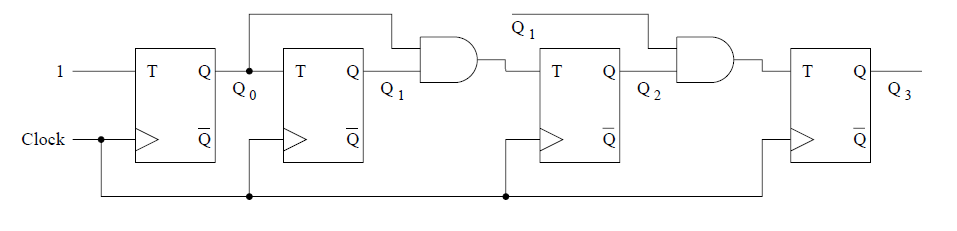
\includegraphics[width=\textwidth]{syncex}
\captionof{figure}{Example of a synchronous digital circuit.  Each output is gated by a flip flop that is controlled by the clock}
%possible picture of clock and flip flops?.... redraw as my own

Asynchronous circuits, as the name suggests, do not depend on a clock. As a result there are varying time delays in its components. The goal of designing asynchronous circuits is to make circuits that achieves some specification in spite of the time delays. That is, irrespective of the time delays, the circuit behaves the same way. One main reason that asynchronous circuits are used is that because it does not require clocks to propagate signals, instead as soon as one logic element finishes the signal goes directly to the next element.  This can allow the circuits to have speedups as it is not waiting for the slowest element for each clock cycle.  The resulting circuit is also very robust as it already accounts for possible variations in manufacturing that contribute to varying time delays.  Additionally even in synchronous systems, small asynchronous circuits are needed to match the inputs coming in from different circuits with different clock frequencies or from the outside world.  For large synchronous circuits clock skew from different parts of the system is also an issue and may be solved with asynchronous methods. \\ %Martin did not give references for these....prob ok then

\includegraphics[width=\textwidth]{asyncex}
\captionof{figure}{Example of a simple asynchronous circuit.  Note that there are no clocks and the signals can propagate at any time}

However, because the signals can arrive at the input at any time, the design is more complicated to ensure that the entire circuit functions correctly.  From a high level view the circuits are designed so that the signals progress irrespective of the delays.  This property is called Delay Insensitivity or Speed Independence depending on the underlying delay assumptions such as the maximum length of delays and on which components.  Even if this is designed correctly, when implemented there can still be hazards.  A hazard is when a certain sequence of delays of the circuit cause unwanted signal transitions to occur.  This may then propogate to other parts of the circuits and cause unwanted behavior.  When trying to eliminate hazards, the underlying delay assumptions are important as well as the implementation details such as gates and transistors. Given the same design under one implementation the circuit may have hazards while under another implemention the circuit will be hazard-free.  Some of the different delay assumptions that could be made are that the delays only occur at gates, or delays only occur on the wires or the delays occur on both gates and wires \cite{myers_book_2004}. Furthermore the bounds on the delay can vary as well. The most stringent case is if we assume that the delay can be arbitrarily long and takes on a value anywhere in the interval $(0,\infty)$ \cite{myers_book_2004}.  Circuits built under the unbounded gates and wires delay model are called Delay Insensitive circuits.  We will not use this delay model because the class of Delay Insensitive circuits is very restricted.  In particular one can only use buffers, inverters, and Muller C-elements to build Delay Insensitive circuits \cite{Martin_1990_DI} \cite{Martin1986_DI}.\\ %2nd reference not necessary 

The asynchronous delay model that we consider is the unbounded gate delay model.  Circuits that can handle any delay under this model are called Speed Independent circuits. The unbounded gate delay model assumes that delays only appear on the gates and the delays can be arbitrarily long in the interval $(0,\infty)$.  The wire delays are negligible.  In addition we assume all forks, which is splitting a signal into multiple branches, do not have any time delays between each of its branches.  These assumptions are reasonable because the delays on the wires only change the operation of a circuit if the wire has forks.  (Otherwise you can lump the wire delay with the previous gate)  When a wire has forks, it is usually true in implementation that the delay between different branches of the fork is less than the delay for gates so that they arrive at the next gates at the same time from the perspective of the relevant gates.  This is also termed isochronic forks.  We focus on the unbounded gate delay model because the delay being unbounded is a pretty harsh requirement and would allow more circuits to work in a real life setting. \\ %how if we assume both gates and wires have delay cannot create many SI circuits, and also Muller is one of the broader classes that we can use

Muller circuits is the approach that D. E. Muller originally proposed based on this delay model \cite{Muller_59}.  Since then a number of synthesis methods following this design has been produced.  Usually the synethsis methods begin with some higher-level specification such as signal transition graph or petri nets and translate into a state graph.  State graphs describes the progression of changes of a finite number of signals.  (The term wires and signals are used interchangeably as the state graph is converted into a circuit.)  Then depending on the underlying implementation, such as generalized C-element and standard C-implementations, the appropriate inputs and logic functions that allows the circuit to function according to the state graph is synthesized.  The end result is a hazard-free and speed independent asynchronous circuit.   
There are other types of delay models and asynchronous circuit synthesis methods such as Quasi Delay Insensitive circuits and the relevant types for this work are described in more detail in the literature review.  \\  %add refs to gen C etc

\section{Organization of this work}
%why are async circuits important, timing delay etc
Because these various faults can interfere with the function of the circuit and even result in harmful operations(catastrophic failures), there has been a lot of work put into making digital circuits fault tolerant. Most of the fault tolerant solutions has been investigated for synchronous digital circuits.  Because the timing difference between different signals arriving do not have to be considered for synchronous circuits, they can use error correcting codes and redundancy techniques such as triple modular redundancy (TMR). Unfortunately many of these techniques have problems if directly implemented in asynchronous circuits.\\

In the rest of this work, in chapter two, I will first introduce the different types of common faults and their causes.  As well as the common fault models that researchers use when investigating these faults.  Then I will go into depth about the asynchronous circuit models that are relevant to this work.  I will then go through the existing body of work on fault tolerant solutions for both types of circuits with an emphasis on asynchronous circuits.  In chapter three, I will show why the existing fault tolerant methods are insufficient and propose a new fault free method for asynchronous transient faults.  I will prove using logical proofs as well as formal verification methods to show why my new method always works.  In the final chapter, chapter four, I will conclude on how to better build fault free asynchronous circuits and suggest some possible new research directions.
%Overview:  why is the problem important  \\  maybe I can extend the Introduction a bit more
\chapter{Background}
\section{Faults}
Faults can be split into permanent and non-permanent faults.  Non-permanent faults are further split into transient and intermittent faults \cite{jha_gupta_2003}. %copied 
A fault is defined as the physical difference between the good or correct system and the current system.  An error may be caused by a fault, which is when the state of the system differs from the state of the good system and thus unable to perform some specified function.  Hidden faults are also possible where the fault does not cause an error \cite{jha_gupta_2003}. \\

Permanent faults refer to the presence of a fault that affects the functional behavior of a system(circuit) permanently.  Some examples that may cause permanent faults are: incorrect connections between integrated circuits, broken components or parts of components, incorrect silicon and metal connections (manufacturing problem), and functional design errors.  Most permanent faults occur during fabrication.  There are many existing literature that cover permanent faults and the different tests at production time that can uncover the presence and location of these faults. \cite{jha_gupta_2003} \cite{giz_book_2006}.  We ignore the possible manufacturing problems and assume that the circuit is free from those problems.  Instead we consider the permanent faults that develop during operation from radiation.  For example, high energy ions can impact the transistors and the circuit causing short-circuiting, rupture of the gate oxide insulation and other permanent faults.\\ %copied from SEE eetimes article

Non-permanent faults is defined as faults that affect the system's functional behavior for a finite but unknown period of time.  They can occur at random moments and are categorized into two types, intermittent and transient faults.  Intermittent faults are caused by non-environmental conditions such as loose connections, deteriorating or aging components, critical timing (hazards and race conditions), resistance and capacitance variations (which may lead to timing faults), physical irregularities, and noise.  Intermittent faults usually affects the system for a shorter time period than the application time of a test developed for permanent faults and thus may not be detected using such a test.  Intermittent faults can transition into permanent faults naturally but may take a long time from hours up to months.  \\

Transient faults are caused by environmental conditions such as cosmic rays, $\alpha$-particles, pollution, humidity, temperature, pressure, vibration, power supply fluctuations, electromagnetic interference, static electrical discharges, and ground loops.  In particular $\alpha$-particles are a major cause of these faults.  These $\alpha$-particles can interact with the semiconductor material which results in the generation of electron-hole pairs. When these $\alpha$-particles collide and interact with the circuit it can induce a voltage/current pulse.  Also known as single-event transients (SETs), if the width of this pulse or transient is wide enough it may propagate through the circuit.  $\alpha$-particles may also interact with a memory element (of which flip flops, latches and C-elements are most relevant to this work) and cause a bit flip in the state of the memory element. This is also known as single-event upsets (SEUs), SEUs include both single-bit and multi-bit upsets but single-bit upsets are most common and much work has been done to eradicate failures from SEUs.  
Transient faults may be hard to detect because it appears sporadically and may not affect the system during testing. \\

In this work we will not be concerned with intermittent faults since it can be thought of as a transition between transient to permanent faults.  Instead the two main fault modes we will look into are transient and permanent faults.  In both radiation effects, also called single event effects (SEEs), figure prominently.  SEEs are an umbrella term that covers the aforementioned SETs and SEUs as well as the single event effects causing permanent faults.  There are two main sources of radiation, one is cosmic rays from space which interact with the atmosphere to produce high energy neutrons.  Another is that $\alpha$-particles can be caused by trace impurities of radioactive elements present in the packaging material of the chip and the silicon substrate.  Radiation from cosmic rays become more severe at higher elevations while the latent source in packaging is difficult to eliminate.  Thus initially a lot of the work in fault tolerant design was done for aviation and space flight.

%failure mechanisms - physical and electrical causes of faults% maybe not that useful... may not need to go in depth

 %digital circuits
%Types of faults transient/perm (and possibly subcases too) \\
%Asynchronous circuits (different types) possibly synchronous too? (and our circuit model based on Meyer) \\
%Then talk about the fault tolerant solutions () \\
\section{Asynchronous Circuit and Synthesis}
In the previous chapter we described how an asynchronous circuit works from a higher level perspective and in particular that it should work under varying delays.  In this section we will cover some definitions and properties of the circuit and also how we can synthesize the circuit from a higher level specification.  Both Speed Independent and Delay Insensitive technologies will be introduced.  There are differences but also many similarities between the two methods.  Even though this work is based on the Speed Independent model, there has been some previous work done on the Quasi-delay Insensitive model so I wanted to provide some context to make a direct comparison.

\subsection{Speed Independent Circuits}
As mentioned in the introduction, the unbounded gate delay model assumes an arbitrary delay on all the gates and ignores any delay on wires.  This delay model is the basis for Muller circuits \cite{Muller_59}.  State graphs describe how we would like the circuit to function.  
Muller circuits are then synthesized from the state graphs.
\begin{definition}A state graph consists of $\langle W, S, T\rangle$ where $W$ is the set of finite signals $\{w_1 .. w_n\}$.  $S$ is the set of functions $[W \to \{0,1\}]$ %<-this might not be right math... and s(k) denotes the (binary) value of the state at signal $v_k$.  
which maps each variable to a boolean.  An element of $S$ is called a {\em state}. $T$ is the transition relation of the state graph, $T \subseteq S \times S$.  \end{definition}

State graphs can also be thought of as each state having a boolean value for each of the signal variables, and states can be named by these values.  For the state graphs that we work with, we assume all states are distinct and that in each transition, only one of the signal values change.  The transition arrows are usually labelled with the signal variable and in which direction the change occurs to help with an easier understanding of the graph. 

\includegraphics[width=\textwidth]{stategraphex}
\captionof{figure}{Example of a state graph.  The order of the variables in each state are x,y}
State graphs can be implemented as an asynchronous circuit where the signals of a state graph $V$ maps one-to-one to wires in the circuit.  Then the set of states $S$ can also describe the state of wires of the circuit.  \\

Next we describe the set of {\em transitions} of a circuit where only one signal value changes more formally.  
We write $s(w)$ for the value of signal $w$ in state $s$, and write $T(s, s')$ when there is a transition from $s$ to $s'$.

A transition has the additional constraint that only one signal is allowed to change between the two states in the transition:
\begin{property}For all $s$ and $s'$ in $S$, whenever $T(s,s')$ holds, there is exactly one $w \in W$ such that $s(w)\neq s'(w)$.
\end{property}
There may be multiple transitions from a state $s$.  A related concept is when the state of a circuit changes when one or more circuit elements is unstable, leading to a change in its output signal.  An unstable element is said to be {\em excited}.


\begin{definition}A wire $w$ in the circuit is {\em excited} in state $s$ if there exists a $s'$ such that $T(s,s')$ and $s(w) \neq s'(w)$. % Alternatively we define a function $f_v$ for wire $v$ such that if wire $v$ is excited in state $s_i$ then $f_v(s_i)$ takes on the value after the excited wire transitions and $f_v(s_i)\neq s_i(v)$.  If wire $v$ is not excited then $f_v(s_i)= s_i(v)$. 
\end{definition} %delete second part if I don't use f_u() later
%For example we propose $f_s$ and $f_r$ as functions that maps the current state to the output of the set and reset blocks respectively.
%(may need to change this definition to s'=/=s) <- added in

Note that from a state $s$ it is possible for multiple wires to be excited as defined above because there may be multiple transitions from $s$ to different states.  Each of the transitions causes a different signal to change.
%[Explain that multiple elements can be excited in the same state because there can be transitions to several different states, and each of those transitions can change a different signal.]
%[Think about including examples: a boolean gate and a C element ]

We consider semi-modular circuits because they are a subset of speed independent circuits and is a large enough class to include some interesting and useable circuits. A simple explanation of semi-modularity is that once a wire is excited, it stays excited until it transitions to the excited value. Formally this can be defined as follows: %proof that semi-modular circuits are also speed independent
\begin{definition}An asynchronous circuit is {\em semi-modular} if for every pair of states $s$ and $s'$ such that $T(s,s')$ holds, and let $v$ and $w$ be wires such that $s(w) \neq s'(w)$ and $w\neq v$, then if $v$ is excited in state $s$, $v$ is also excited in state $s'$ \end{definition}

%ADD SPECIFIC CONDITIONS THAT ALLOW SYNTHESIS
When the state graph have the following properties, it is possible to synthesize a hazard free and speed independent asynchronous circuit following the state graph.  Each variable from the state graph is implemented as a gate logic that takes other variables/wires as inputs and outputs a variable/wire.  We next look at how such a gate logic can be made.\\ 

%C-elements
The C-element proposed by Muller is an important building block for asynchronous circuits.  It acts as a memory element in that it receives two inputs.  When both inputs are low, the C-element output goes low, and when both inputs are high the C-element output goes high.  However when the inputs are mismatched then the output gets held at its previous value.  This can be achieved in a number of ways such as a gate implementation as well as a transistor level implementation with feedback using a weak transistor, other implementations use capacitance to achieve this weak feedback.
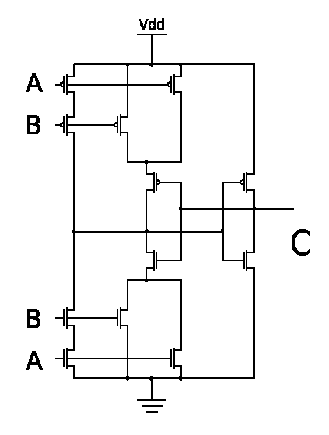
\includegraphics[width=\textwidth]{celement}
\captionof{figure}{ a. logic of the C-element. A, B are inputs, C is the output \\  b. diagram of a C-element at the gate level   c. transistor-level implementation}

C-elements can be used in various asynchronous circuit designs and is an essential component of Muller circuits.  \\

The two specific Muller circuit implementations that we consider are the generalized C-element and standard C-implementations.  We assume that the circuits we want to make fault tolerant follow these implementations.    
For each wire in the state graph there is a gate logic that controls the value of the wire.  We look at two conditions, set, the condition for the wire to transition to a high value; and reset, the condition for the wire to transition to a low value.  The gate logic then implements the set and reset conditions. The details of how this is implemented is that we use the state graph to generate the set and reset conditions. For each set and reset there is an ON-set, OFF-set and Don't Care set.  ON-set are all states in the state graph where the wire is excited and a transition will occur.  That is for the set condition, it must evaluate to TRUE for these states so that the wire can transition to high.  OFF-set includes all states where the set condition must evaluate to FALSE which is the states where the wire is excited but to the opposite value, which is low for set, as well as all states in the state graph where the wire value is at the opposite value, again low for set.  The rest of the states are in the Don't Care set which includes states that are not included in the state diagram.  It does not matter what the set condition evaluates to in these states as they do not disturb the function of the circuit. The same procedure applies as well in finding the ON-set, OFF-set and Don't Care set for reset except substituting in reset for set and flipping the value of the wire where needed. The set and reset conditions then must include all states in the ON-set and not include all states in the OFF-set so that the wire transitions according to the underlying state graph.  The set and reset can be implemented separately with logic and the gate logic for the wire includes logic for both set and reset and also the combination of them into the output wire.   \\   %Beerel and Myers.... also expand? 

Even though the generalized C-element is presented as a C-element with set and reset as inputs, the transistor level implementation differs slightly.  We assume a transistor level implementation of the set and reset combined with the C-element so that there is only one delay for the entire logic block.  In addition this is not a normal C-element because set is used exclusively for the pull-up logic and reset is used for the pull-down logic.  In a normal C-element we allow for any four combinations of the values of the set and reset input wires.  However using the pull-up and pull-down logic setup, we do not allow for when both set and reset is `ON' as the output wire would simultaneously be connected to the high voltage and ground.  Such an output would have indeterminable voltage values and violate the digital assumptions.  Thus, the set and reset logic is designed so that they cannot overlap.  This corresponds to $\overline{set}\vee\overline{reset} $ is always TRUE.\\
\begin{center}
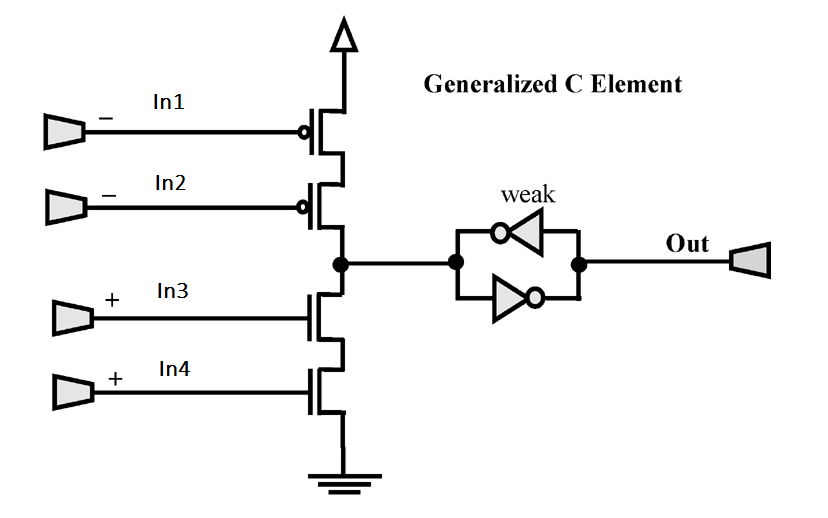
\includegraphics[width=.7\textwidth]{genC}
\end{center}
\captionof{figure}{transistor level implementation of a generalized C-element.  The + signs are the set logic inputs and - signs are the reset logic inputs.  For this particular element, set is in3 AND in4 while reset is in1 AND in2.}

The main difference is that the set logic and the reset logic must be designed so that they do not turn `ON' at the same time.\\

For the standard C-implementation, we allow for more variation in delay.  For the gate logic of each variable in the state graph, we look at the set and reset logic as composition of various gates (such as AND, OR, NOT).  Each of these gates can have their own delay that is arbitrary in length that is instantized as an intermediate wire.  Thus the logic must be synthesized more carefully to eliminate hazards that can occur in these intermediate wires.  In particular the set and reset must be activated at states only when the wire is appropriately excited.  As a result, the standard C-implementation has a number of set logic functions combined by an OR gate and fed into one input of the C-element.  There will also be a number of reset logic functions combined by an OR gate and passed through an inverter and fed into another input of the C-element.  This implementation uses the standard C-element so that if the set and reset inputs are mismatched, the output is held.  In general the synthesis can be changed so that there is a hazard-free implementation using only two-input gates.
 
 %explain sop?
 
 \subsection{Quasi Delay Insensitive Circuits}
 %QDI
Quasi Delay Insensitive Circuits (QDI) are related to Delay Insensitive Circuits.  Previously we mentioned that Delay Insensitive circuits operate under the assumption that both the gate and the wire have unbounded gate delays.  In particular each branch of a fork will have different delays and can be treated as separate wires.  One result about Delay Insensitive circuits is that it is a very restricted class.  Instead if that condition is relaxed so that some of the forks are allowed to be isochronic, then a more general class of circuits can be constructed.  Note that in the case where all forks are isochronic, then this becomes the same as speed independent circuits.  \\
 
The gates of a QDI circuit is formed from Production Rules (PRs).  For the single output case, a gate takes a set of variables as inputs and outputs a variable.  Again a transition on the variable $x$ is denoted as $x\uparrow$, a transition from $x=0$ to $x=1$; and $x\downarrow$, a transition from $x=1$ to $x=0$.  Then the two PRs associated with the gate with output $x$ is :
\begin{align*}
   B_u\mapsto x\uparrow \\
   B_d\mapsto x\downarrow 
\end{align*}
Where $B_u$ and $B_d$ are called guards.  Each guard is a boolean condition formed by some combination of the input variables.  When a guard is evaluated to be $True$ then the transition is activated.  When it is $False$ then the corresponding transition does not happen.  Note that similar to the generalized C-elements, both guards cannot be active at the same time.  In addition it is assumed that each guard is in a sum of products of the input variables.  The PRs of a circuit are evaluated all at the same time.  At any point in time, if a transition is activated, it will transition in a finite amount of time as long as the corresponding guard is held at $True$.  This is due to the assumption of the arbitrary delay of a gate.  Note that again, like the generalized C-element implementation, we assume that the transistor level implementation of a PR allow any arbitrary sum of products to be made where there are no delays within the logic of the sum of products.\\

Another important property of QDI circuits is \textit{stability}.  A guard is stable if it evaluates to False after the transition of the output variable is complete.  This eliminates any hazards that may arise when a guard is True and before the output has fully transitioned, the guard then evaluates to False and the transition is terminated.  This may cause a blip in the voltage, an incomplete transition, where the circuit may interpret it as either no transition or two consecutive transitions.  One additional assumption is that the PRs cannot be \textit{self-invalidating}.  That is, when a transition on an output occurs, it cannot immediately falsify the guard.  With this assumption, it can be shown that the output of a gate cannot also be its own input variable.  There are no self-loops.  

\section{Fault Tolerant solutions}

%soft error protection <- error correcting codes for SRAM memory
Because faults cannot be eliminated in digital circuits, different methodologies have been used to make the circuits fault tolerant.  Much of the research done in this area are for synchronous circuits.  There has also been some research for asynchronous circuits using some similar techniques. First we present an overview of some common techniques for synchronous circuits, then introduce the current techniques for asynchronous circuits.  Some of the techniques in asynchronous design borrows or are inspired by the much more developed fault tolerant synchronous circuits field.  However due to the difference in timing assumptions of the two types of circuits the techniques are not completely transferable.  We describe why some of the solutions from synchronous circuits cannot be directly applied to asynchronous circuits.\\

%- used in the early days for space and flight, and systems that CANNOT go offline/errors like stocks and banking.
%- different techniques... explain a bit about each
%-hardware, software, hybrid, 
%-detection vs correction
%- ECC/ parity checking (needs software/ controller) (Mitra's method)
%-TMR is still super important (possibly why TMR is not viable for async)
In the early days there were certain systems for which eliminating faults and errors were very important.  These include space and aviation control systems where due to the altitude there are more radiation and thus more faults.  In addition faults that cause error is very detrimental to these systems and may cause failures leading to loss of life.  Other examples of systems requiring reliable circuits include banking and stock market applications where the system must function without error for hours at a time and in case of any error may have devastating consequences, such as a bit flip of the most significant bit in a money transaction. \\

Solutions for eliminating these transient fault induced errors include physical, hardware, software or a mix of the previous.  Some commonly used techniques are transistor sizing, circuit hardening, hardware duplication, and time redundancy \cite{Mitra_08_softerrors}.  Transistor sizing is a physics based technique and does not reduce as much soft errors as the other techniques.  Circuit hardening is on the physics level, where it uses intrinsic properties such as resistive or capacitive hardening, or combining the transistors differently to have less effects from transient faults. (?)  Hardware duplication, is a common technique that tries to eliminate soft errors on the circuit level.  This is achieved by having multiple duplicates of a circuit and often comparing the value from each duplicate to find and eliminate errors.  For example Triple Modular Redundancy (TMR) has been used since the beginning of the field and is still a good solution for eliminating single soft errors.  The advantages are that it is able to eliminate nearly all soft errors but also due to the duplication, the area for each circuit and additional power increases substantially (correlates to the number of additional duplicates).  Time redundancy techniques re-use the same circuitry to compute values multiple times to ensure there is no error.  This technique is not completely hardware based and requires software to manage re-using the same circuity with the same inputs over time.  The area of the circuit does not change but the speed of the circuit worsens substantially. \\

There is also the additional distinction between error detection versus error correction.  In general it is easier to detect an error than to correct it.  For example using hardware duplication, only 2 copies are required to detect an error but 3 copies (TMR) to correct the error.  For different parts of the system there are also different strategies.  For example in memory components such as SRAM, soft error correction is usually done using error-correction codes.  These codes are compared to the bits that are stored to ensure that there are no errors.  They are designed to handle a predefined maximum number of errors.  For example Hamming codes where each codeword are at least a distance of 3 apart can handle one error.  This method is not purely hardware based and a controller system and software is used to match the codes and detect and correct any errors.  For a control circuit, there are also a variety of strategies.  Again, one could make use of error correcting codes or parity bits to detect or correct errors in combinational logic \cite{McCluskey_99}.  This uses a combination of hardware and software.  A completely software approach is to run a program on some input, then run the program again on a transformed version of the input where the output can be mapped back to the original output \cite{Mitra_softwareerror}.  If the output and the transformed output do not match then the fault is detected.  Lastly, for hardware only methods, even now TMR is a commonly used method because of its robustness and ensures error correction. \\
%However these cannot be used for latches or flip flops.  In these circuits,    Some of these techniques only detect errors but do not correct them.\\

Triple Modular Redundancy is a technique where each combinational logic unit is copied three times and then fed into a latch that performs a majority voting operation.  That is, if at least 2 out of the 3 signals agree on a value, the output becomes that value.  Additionally, to counter possible faults on the single output wire, the majority vote unit can also be copied three times and it's output wire fed appropriately as input to the three copies of the downstream combinational logic.  This would resolve both transient and permanent single faults.  However the downside is that the circuit needs to be copied three times so the area is three times larger and the power consumption as well.  In addition there must be many adaptations for this to work in asynchronous circuits as the signals can arrive in different orders.  We give an example of why TMR does not work in an asynchronous circuit as it does in a synchronous circuit below.  We assume that in the original circuit that each logic block has some input wires and an output wire.  In the TMR scheme, each logic block is triplicated and to remove single points of failure, we also triplicate the majority voter that the three copies of the output wire feeds into.  There are also three distinct copies of each input signal that correspond to outputs from the three voters.  This is the basic scheme that synchronous circuits with TMR uses.  Because this circuit is asynchronous, we assume that each logic block is composed of gates that has some arbitrary delay that is independent of other gates.  This is true under both delay assumptions of speed independent and delay insensitive circuits.  We ignore whether a fault can be in the voter for now. 
\begin{center}
\includegraphics[width=\textwidth]{tmrcounterex}
\end{center}
\captionof{figure}{An example of an error if a fault occurs in an asynchronous TMR circuit}
Initially all output wire values are `0's.  Then since the input signals are distinct copies of each other, it is possible for one set to finish transitions (new) before the other two sets and the first logic block transitions to a `1'.  Then a transient fault arrives on the output of the second logic block which transitions to a `1' as well.  The majority voter would then transition to a `1'.  However the upset from transient faults usually happen within a short time period and the old inputs eventually force the output of the second logic block back to `0'.  Then the majority voter would transition to a `0' so that causes a hazard on the output of the majority voter.  %depends on if the logic gate was combinational logic.... which I guess we can assume it is
%NEEDS FIXING AND CHECKING
It is also possible for the `1' from the majority voter to feed into other logic units which is effectively an early transition.  That early transition will then put the circuit into states that are not specified by the original state graph and thus the next states cannot be predicted.
\\

%also included detection schemes because there is so few works in the literature...
David and Ginosar (1995) prove that a specific type of asynchronous circuit called self-timed combinational logic is self-checking under stuck-at-faults \cite{self_timed}.  (Stuck-at-faults are permanent faults where a wire value is stuck at 0 or 1)  That is if there is a single stuck-at-fault, the circuit will either stall or give an illegal output so that faults can be detected.  Each input and output is encoded by 2 bits also known as dual rail encoding.  10 represents 0, 01 represents 1, and 00 represents undefined or the system is not yet ready.  11 is an illegal output that only occurs under certain faults.  Each logic unit is composed of four subunits, three of which control the inputs and outputs and includes many C-elements.  The fourth one implements the combinational logic.  The combinational logic requires the implementation to be such that each output bit is monotonous given the input bits.  A further restriction is that the combinational logic is composed of only AND and OR gates.
\\

Verdel and Makris proposes that simply porting the duplication strategy for error detection from synchronous circuits does not work for asynchronous circuits \cite{async_dup_ced}.  This is because the duplication strategy relies on both the original and duplicate to output the same value.  Some modifications that they propose to make the duplication error detection strategy work is to assume additional timing requirements.  That both copies should output the same value within a certain time determined by a pre-set delay element.  Everytime one of the signals transitions to a new value, and the duplicates are mismatched the timer starts and if they stays mismatched when the timer ends an error is detected.  They look at stuck-at-faults and premature firing faults.  There are also cases when the timer detection does not work and for those cases they propose using additional hardware to look at the states of all the wires to see if an illegal state was reached.  They present an example of a control circuit for data computations.  The main restrictions of this method is the additional timing assumptions they make about two copies of a circuit, and that the extra hardware components are assumed to be fault-free.  Also it requires an additional comparison unit for each pair of signals which may be costly.  Only one copy of the duplicates produce output signals that interfaces with the other units so that if there is an error on that signal it is not detected until some time after the error has propagated.
\\

Almukhaizim and Sinanoglu (2007) propose a Triple Modular Redundancy (TMR) based method of solving transient errors but requires a hazard-free majority voter.  Transferring the TMR method that solves faults for the synchronous circuits to asynchronous requires the change that 2/3 copies agreeing is not good enough but 3/3 is needed to propagate a signal.  This is due to the asynchronous property where signals can change at any given time and thus one signal changing plus a transient error may cause the output wire to transition prematurely.  For permanent errors there is an additional problem of deadlock and this configuration does not solve it completely. \\
\\
In the paper by Manohar and Peng (2005), they add in new circuitry that solves faults for a specific asynchronous adder circuit \cite{PengManohar_asyncadder}.  The faults that they consider are fabrication defects, permanent faults and unrecoverable failures.  New nodes and edges are added to make it k fault tolerant.  They detect when there is a deadlock at which time it reconfigures the circuit by trial and error of all the possible combinations until the circuit is no longer deadlocked.   \\

Naqvi (2014) shows how to solve transient faults on muller pipelines \cite{Naqvi_mullerpipeline}.  Muller pipelines make use of handshaking protocols.  The assumptions they make are that only one fault occurs per handshake cycle.  They used formal verification to show that it works for one pipeline component. \\
\\
Jang and Martin (2005)’s paper considers the problem of single SEUs in QDI circuits \cite{JangMartin_SEUQDI}.  In the original functioning circuit, an SEU may cause a) a transition to a deadlocked state, an illegal state with no further possible transitions, b) abnormal, a transition to another state in the state graph and skip or adds certain transitions/signalling, c) tolerant where it transitions to an illegal state but the PRs are unaffected and eventually resumes to a valid state in the state graph.  They solve this problem by duplicating the circuit and appending C-elements to the end of each of the original wires .  In addition to duplicating the circuit they change the production rule set so that if the rule is about wire $X$ is true in the original circuit, in the new circuit the rule is $X^1$ and $X^2$ both have to be true.  For example
\begin{align*}
   B_u (...,x,...)\mapsto z\uparrow \\
   B_d (...,\lnot x,...)\mapsto z\downarrow
\end{align*}
after duplicating the circuit and adding in C-elements becomes:
\begin{align*}
   B_u^{double} (...,x_a\wedge x_b,...) & \mapsto z'_a\uparrow, z'_b\uparrow\\
   B_d^{double} (...,\lnot x_a\wedge \lnot x_b,...) & \mapsto z'_a\downarrow, z'_b\downarrow\\
   z'_a \wedge z'_b& \mapsto z_a\uparrow, z_b\uparrow\\
   \lnot z'_a\wedge \lnot z'_b& \mapsto z_a\downarrow, z_b\downarrow
\end{align*}
The last two production rules correspond to the additional C-elements added.  
They prove that with this new circuit, single SEU errors do not cause transitions to deadlocked states, nor abnormal transitions and thus are corrected.  Given the transistor-based QDI assumptions, any changes to the production rules are implemented at the transistor level and assumed to not add any delays.  In addition QDI logic is implemented in sum-of-products form and the production rules are excited only in the appropriate non-illegal states.  Faults are assumed to occur on the input/output wires as well as the new wires that feed into the C-elements.  Another assumption is every loop in the control circuit is at least length 3 to prevent deadlock. %not sure about this, may only be relevant for when they don't double the inputs
\\

The circuit transformation that Jang and Martin proposes work for their assumptions and specific implementation of QDI circuits at the transistor level.  However it is not reasonable to assume that any PR can be implementation with transistors with no delay.  Also for a simple 2-element inverter circuit their transformation also can end up in a deadlocked state after an SEU.  After the duplication and addition of C-element.  
\begin{center}
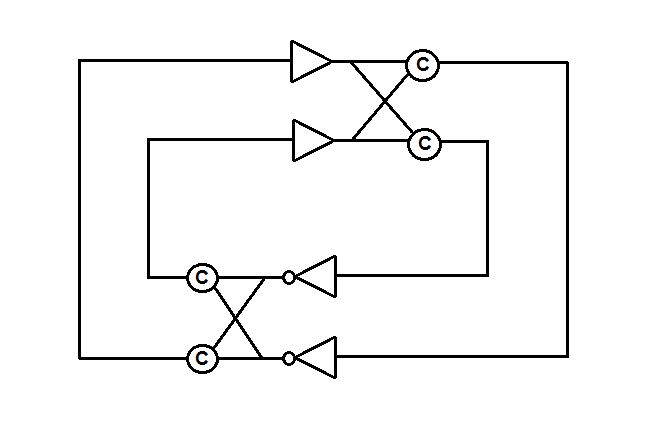
\includegraphics[width=.7\textwidth]{transfex}
\end{center}
Then if a 0->1 SEU occurs at $c_1^B$, it is possible for this circuit to deadlock.
\begin{center}
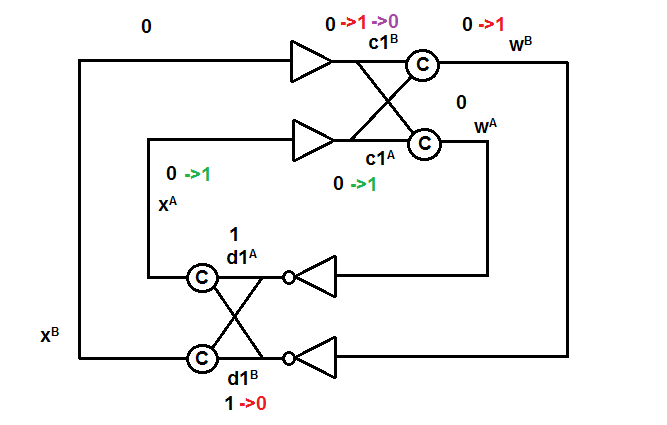
\includegraphics[width=.7\textwidth]{transfexc}
\end{center}
%fix later... it's technically that a simple duplicate and C-element scheme does not work

In some of the previous work they make additional assumptions such as the checking circuit is fault free.  We propose an asynchronous circuit transformation on a more general type of circuits, control circuits.  The transformed circuit can function under single transient faults.  In addition, we assume a gate level model of the circuit and allow the transient to occur on any of the wires thus solving the transient fault problem for a bigger class of circuits.


\chapter{Fault Tolerant Circuit Under Normal Operation and Single Transient Fault}
\chaptermark{Fault Tolerant Circuit}
\section{Traces and circuit equivalence}
We solve the problem of single transient faults by taking a semi-modular circuit (the original circuit) and applying a transformation to the circuit by duplicating all its circuit elements.  Due to the asynchronous nature of how signals are processed, corresponding wires in the resulting half circuits may have different values.  To solve this problem we add C-elements to synchronize the two versions of the same signal.   An example of this transformation applied to the simple inverter circuit is shown in figure \ref{fig:dupschemeex}.  Both the duplication and the additional C-elements configuration are shown.  In the rest of this chapter we define a way to compare two circuits and to show their equivalence.  Then we propose our transformation method and show that under normal operation (no faults), the fault tolerant circuit is equivalent to the original.  Finally we show that if a single transient fault occurs, one side of the fault tolerant circuit is equivalent to the original and we can still extract the signals that we desire.\\
\begin{figure}
  \centering
    \includegraphics[width=.9\textwidth]{transf3Csimp}
  \caption{a) original circuit b) after the fault tolerant transformation}
  \label{fig:dupschemeex}
\end{figure}

Other than the basic terminology for asynchronous circuits, we also want terminology to compare two circuits based on their function.  
We first define a {\em trace}, to describe a path the circuit can take as it follows the state graph.  Different paths can occur because there may be multiple transitions from each state.  We call the succession of states and transitions the trace which is defined as follows:
\begin{definition}A {\em trace} $\sigma$ of a circuit is a sequence of states of finite or infinite length and $s_i$ is the $i^{th}$ term of the sequence.  %Formally this is written as $\sigma: 0,\ldots ,n-1 \to S$ and $n \in \mathbb{N}$.
 Also every pair of consecutive states in a trace are transitions% such that $T(s_i,s_{i+1})$ for $ 0\leq i\leq n-2$
 .  We also use the $\sigma_n$ as shorthand to denote the sequence of the first n states of $\sigma$\end{definition} 
Thus a circuit has a set of traces.  
A circuit also has a set of initial states where the traces can begin in.  The set of initial states are the same as the set of states in the state graph.\\

%Note that our definition of trace also includes the case where there is only one transition from each state of a state graph, which results in a linear state graph.  

\begin{figure}
  \centering
    \includegraphics[width=.6\textwidth]{sm_counter2}
  \caption{a) original circuit for wire w b) an erroneous initialization}
  \label{fig:sm_counter2}
\end{figure}

The original circuit is semi-modular by design.  But the design only covers cases where the wires are in a state in the state graph.  That is, hazards may occur if the circuit goes into an unreachable state of the state graph and the circuit is no longer semi-modular and furthermore becomes unpredictable.  This does not happen in the fault-free case where the circuit is initialized to a state in the state graph and the wires inside the logic blocks are properly initialized.  However when faults do occur, the circuit may become unpredictable and a reason why we need to transform the circuit to protect against faults.  An example of what might happen when the circuit is not in a semi-modular state is shown in figure \ref{fig:sm_counter2}.  The logic circuit for wire $w$ is taken out of a semi-modular circuit.  However, if the state of the $w,x,y,z$ wires are $(0,1,0,1)$ and the internal wires after the AND and OR gate are both initialized to 1, this is not semi-modularity consistent.  The output wire $w$ is excited to 1 while the inputs from $x,y,z$ will cause $w$ to transition to 0.  Depending on the timing of the gates, $w$ may stay at 0 or experience a glitch to 1 then back to 0.  The extra layers of gates in the logic block can be thought of as extra delays that can store and propagate the wrong values.  More detailed discussion on how to initialize and keep the circuit semi-modular is explored in the subsequent section.\\

Given two circuits, how can we determine when their basic functionality is the same, especially if they are implemented with different gates and circuit elements?  We define a notion of equivalence between two circuits through their sets of traces.  
%We want the underlying state graph representation of the circuits to be equivalent.  However only the signals and the sequence of transitions from the circuit is observable.  In other words the trace is observable.  Thus we define circuits as equivalent if the set of traces of the two circuits are the same. [We use the assumption that if the set of traces are equal then the state graph is equal.]
\begin{definition} Two circuits A and B are {\em equivalent} if the set of all traces from circuit A is equal to circuit B.  In other words, $\{\sigma^A |\sigma^A$ is a possible trace in $A\}=\{\sigma^B |\sigma^B$ is a possible trace in $B\}$.
\end{definition}

We are now ready to explore how to make a circuit fault-tolerant.
%good enough for now, do I need if and only if? <-NO, xxx if xxx in math lingo is iff

%An additional property of the asynchronous circuit is that one can view each wire as a separate black box.  For a wire $v$, inputs from the rest of the circuit ($I_v$ and $I_v \subseteq$ V) feed into a gate and outputs the wire value $v$.  We call the instantaneous value of the gate for $v$ of a state $s$ as $f_v(s|_I)$, where f is the function $f:[I \to \{0,1\}] \to \{0,1\}$ and $s|_I$ is the state $s$ projected on the input variables $I_v$.  If inputs to the gate remain constant, the output $v$ will eventually take the value specified by $f_v(s|_I)$  %maybe change v again, also the f(s) vs f(I) thing...
\section{Fault Tolerant transformation}

We can make an existing semi-modular circuit fault-tolerant by the following transformation as shown in figure \ref{fig:dupscheme}: make a duplicate copy of the logic blocks of each wire $w$ and label the duplicate wires $w^A$ and $w^B$.  We also label the duplicated logic blocks as belonging to circuit A or circuit B in agreement to the wire naming.  Then we connect the output of the logic blocks to three layers of C-elements as shown in figure \ref{fig:dupscheme}.  We label the intermediate wires as $c1^A$, $c2^A$, $c3^A$ for circuit A and $c1^B$, $c2^B$, $c3^B$ for circuit B.  In the first layer of C-elements, $c1^A$ and $c1^B$ are outputs of the logic blocks and inputs to two C-elements outputting $c2^A$ and $c2^B$.  These are then the inputs to the second layer of C-elements outputting $c3^A$ and $c3^B$.  These are then the inputs to the third layer of C-elements outputting $w^A$ and $w^B$.  We can label one of the final C-element outputs as $w^A$ and the other output as $w^B$.  These then connect to other logic blocks in circuit A and circuit B respectively.  Note that when labelling the C-elements and its outputs, which side is A and B can be somewhat arbitrary because the output pairs are symmetric.  The symmetry is broken when connecting the final output wire $w^A$ to all the circuit A gate inputs and wire $w^B$ to all the circuit B gate inputs.  All circuit elements with the A label is part of the A-half circuit and all circuit elements with the B label is part of the B-half circuit.\\%(Note that the outputs of the C-elements can be arbitrarily named and connected to the next gates, and the next gates can also be arbitrarily named $A$ or $B$ as long as it does not create any inconsistencies in the naming convention, ie. all $A$ wires feed into the $A$ gates)  %the only wires that really matter are the wires that have isochronic forks, these must input to same A or B, everything else is just a naming difference
\begin{figure}
  \centering
    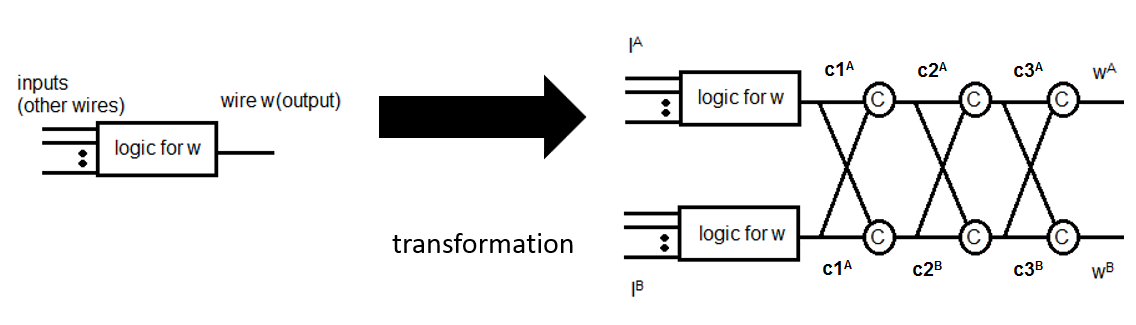
\includegraphics[width=\textwidth]{circuitforproof3}
  \caption{Fault tolerant transformation: duplicate the original logic for each output wire and adding 3 layers of C-elements}
  \label{fig:dupscheme}
\end{figure}

We want to show that a half circuit from the fault tolerant circuit has correct function.  To do this, we define a correspondence between states of the original circuit and states of the fault tolerant circuit.  As a result of the circuit transformation, a state of the fault tolerant circuit has bits for 8 times as many wires as a state in the original circuit.  Half of those bits are obviously from the A half and half are from the B half of the circuit.  The state graph for a fault tolerant circuit is defined on this combined state.  We define the half-circuit mapping $h^A: s^{\mathit{full}} \to s^A$ where $s^{\mathit{full}}$ is the combined state of a fault tolerant circuit and $s^A$ consists of wires $w^A$ that correspond to the original wires $w$ in the original duplication procedure.  The half-circuit mapping $h^B$ is similarly defined to map $s^{\mathit{full}}$ to $s^B$.  The added wires such as $c1^A$, $c1^B$, $c2^A$, $c2^B$, $c3^A$, $c3^B$ from the duplication procedure are hidden by $h^A$ or $h^B$.  We extend $h^A$ to traces by using the following two steps: first, $h^A$ is applied individually to each state in a trace $\sigma$, and likewise for $h^B$.  %not sure if I want the mapping to be from variable to variable or specific state to state
%For a trace in the fault tolerant circuit we project the full states onto a shortened list of wires (ie the wires corresponding to the original circuit). 
The resulting trace may have successive repeated states.  So we delete all but one of the neighboring repeats to obtain a valid trace on the shortened list of wires.  The result should be a trace from the original circuit.
 Using this mapping we will show that the original circuit is equivalent to half of the fault tolerant circuit in both the absence and presence of a single transient fault.
%do I need to define all the new transitions in duplicated circuit?  maybe
\\

%[Why is this the best we can do?]
We compare each half circuit because it is not easy to synchronize and compare the signals between both halves, especially if we reuse the logic blocks from the original circuit.  A simple idea we tried was to insert another C-element before the input is fed into the logic, to synchronize the wires on both halves.  The problem with that is in the original circuit, a wire value change propagates to all inputs at the same time.  Adding another layer of C-elements creates delays at the input to logic blocks and the isochronic fork assumption is violated.  Thus the resulting circuit will not function according to the specified state graph.  (an example can be provided but not sure if needed?)\\  
\begin{figure}
  \centering
    \includegraphics[width=.8\textwidth]{counterexhalf}
  \caption{State graph example to show how b can transition before a or c finishes in both halves in the fault tolerant circuit}
  \label{fig:counterexhalf}
\end{figure}

Next we look at the traces of each half circuit.  Figure \ref{fig:counterexhalf} shows a subsection of a semi-modular state graph where each state is given a nominal name (state 0, state 1, ... etc) and each transition is labeled with the transitioning wire.  Suppose we apply our fault tolerant transformation to such a circuit based on this state graph.  Both halves in the fault tolerant circuit will transition based on this state graph, with the added caveat that for a wire to transition at some state, it must be excited in both halves.  Starting in {\em state 0}, it is possible for the A-half to transition to {\em state 1} ($a^A$ transitions) and for the B-half to transition to {\em state 2} ($c^A$ transitions).  We assume that $a^B$ and $c^A$ do not complete their transitions yet.  Immediately, in the A-half, $b^A$ is excited and in the B-half, $b^B$ is excited.  Then, suppose the transition on wire $b^A$ and $b^B$ occurs.  That is, the A-half transitions to {\em state 3} and the B-half transitions to {\em state 5}.  And finally, the excited $a^B$ and $c^A$ transitions so that both halves are in {\em state 6}.  The trace so far for the A-half is (state 0, state 1, state 3, state 6) while for the B-half it is (state 0, state 2, state 5, state 6).  Thus the two halves need not have the same trace.  One criticism may be that the current fault tolerant transformation synchronizes at the outputs of the logic blocks.  If we want to reuse the same logic blocks but synchronize the signals earlier, such as replacing the final C-element in a standard C implementation with a 4C-element, the issue of different traces in the two halves will still occur.  We have already shown earlier that synchronizing the input signals while keeping the original logic block also can result in error.  This points to looking at properties of each half circuit as the right thing to do.\\ 

Another problem that the fault tolerant transformation cannot resolve is that if we take the following view for transitions, a transition of wire $w$ in the original circuit is complete if both $w^A$ and $w^B$ transitions in the fault tolerant circuit, then some signals may transition out of order.  We use the earlier example of figure \ref{fig:counterexhalf} to show this as well.  Following the same transitions outlined above, $b^A$ and $b^B$ can finish their transitions before $a^B$ and $c^A$ transitions.  Then the $b+$ transition is actually completed before $a+$ or $c+$ and the combined trace no longer maps back to a valid trace in the original state graph.  Another approach we may take is to record the first transition of a wire in either half of the fault tolerant circuit.  For example, if $w^A=w^B$ and then $w^A$ transitions, we map this to a transition on $w$ in the original circuit.  This approach ensures the resulting trace is a trace in the original circuit (can be shown by Lemma 1 and Lemma 2.1 in the next section), however, in the presence of faults, it is easy to see that it does not provide any fault tolerance.\\

For the aforementioned reasons, we choose to use the $h^A$ and $h^B$ mappings and compare each half circuit against the original circuit.  Out of the various comparisons methods and circuit transformations that we tried, it is the most reasonable and results in some nice properties.  We will next demonstrate that the half circuits are equivalent to the original circuit in the absence of faults.  Then we show that a similar property is true even when a single fault may occur.



\section{Normal operation analysis}
To prove claims about the fault tolerance of this circuit, we first prove that the circuit behaves similarly to the original circuit under normal operation.  That is, the set of traces of the fault tolerant circuit after applying a mapping of $h^A$ is equivalent to that of the original circuit.  And likewise after applying a mapping of $h^B$ to the fault tolerant circuit.  We show this through several Lemmas. Lemma 1 shows for each fault-free half of a circuit, if a transition occurs, it must be a transition in the state graph of the original circuit.  This is a strong result; it is true for arbitrary behavior of
signals in the other half circuit, so long as those signals are well formed Boolean values and also does not cause the fault-free half to deviate from well formed Boolean values.  
This result is also significant later in proving fault tolerance under a single transient fault since one of the halves is fault-free.  %as long as it does not violate digital abstraction
%One additional assumption that we make about the gates and wire values (including in the presence of faults) for Lemma 1 to hold is that wire values are strictly 0 or 1, and transitions from excited gates also only produce 0 or 1 and no in between values, no matter the duration of signals from the input wires.
\\

Note that Lemma 1 allows for the possiblity of deadlock.  Lemma 2 shows deadlock does not occur during normal operation.  Combining these two Lemmas, we can show that all traces in the duplicated circuit can be mapped to a trace in the original circuit.\\
% and all traces in the original can be mapped to duplicated after h mapping?  <-this is obvious though by setting the A half and B half to both transition according to original trace
%[so no deadlock in normal operation??]

Now we will discuss the proper wire initializations before going into the Lemmas.  In normal operation, the fault tolerant circuit must have wire values consistent with semi-modular behavior in the original circuit.  
This includes the internal wires which exist in the logic blocks in the original circuit and through duplication also exist in the fault tolerant circuit.  The actual values of these wires do not matter if the inputs to the logic blocks follow the semi-modularity property, and if the internal wires are initialized properly.  This arises from the original synthesis method to synthesize the circuit from an underlying state graph.  
Additionally, it does not suffice for the inputs to the logic blocks to be from a valid trace of the state graph; the timing matters as well.  The semi-modularity property must be preserved:  if the logic block output is excited then it must remain excited until a transition on its output occurs.  Since certain inputs which are valid states and arise from valid transitions may cause the logic block to become unexcited before a transition occurs and thus break the semi-modularity property, we require this more stringent criteria.  %maybe needs an example
Thus to satisfy semi-modularity, the inputs wait at certain input states until the output transitions.  Then the internal wires of the logic block are termed {\em semi-modularity consistent} if the following properties are true:  if the inputs follow semi-modularity then there are no glitches at the output; and once the output is excited it remains excited until the output transitions. \\%newly added

What values to initialize the wires of a circuit to is very important.  We want certain properties to hold for all states that the circuit goes through, and such properties must also hold for the initial state.  On one hand, the initial state $s$ must be a state in the underlying state graph.  Thus the wire values is initialized to be consistent with that property.  On the other hand, as mentioned previously, the internal wires at the initial state (and each state thereafter) must be semi-modularity consistent.  We assume that we can initialize the wire values of the original circuit to satisfy these two properties.  Given this, we pick convenient initializations for the fault tolerant circuit.  The following procedure covers how to initialize both the wires from the duplication as well as the extra $c1^A$, $c1^B$, $c2^A$, $c2^B$, $c3^A$, $c3^B$ wires that are introduced.
%For all initial states we assume that we know the values of every wire in the circuit, intermediate and visible wires.  The visible wire values are the output wires in the circuit $w$, and the wires $c1$, $c2$ and $c3$'s. The intermediate wires are all other wires, which consists of all the wires within the logic blocks for each output wire.  Given these we will show how to define a corresponding initial state in the duplicated circuit.  %should I delete intermediate?
\begin{definition} A {\em valid initial state} for the A half of the fault tolerant circuit is constructed as follows.  Given any state in the original circuit state graph $s \in S$, assume that there exists initial wire values that correspond to $s$.  In addition, for each wire $w$, the internal wire values within the logic block of $w$ are semi-modularity consistent.  Construct the valid initial state by copying the internal wire values to corresponding internal wires in the A half circuit.  Then assign the value $w$ to appropriate wires in the A half circuit such as $w=c1^A=c2^A=c3^A=w^A$. The same construction can be applied for the B half circuit as well.
\end{definition}
%\textbf{
This is one out of many possible initializations that can fit the behavior we want.  Thus this definition is stronger than it needs to be but is used for the sake of conveniece.  In Lemma 1, we will show why this definition allows for the behavior that we want in the fault tolerant circuit.\\

To avoid overly clunky sentences, we will assume that fault tolerant circuits start from the same valid intial state in both halves.  One exception to this assumption is Lemma 1 where only one half circuit is needed to start from a valid initial state since the property is true regardless of the wire values of the other half.\\ 
%For all subsequent discussion in this document, when we talk about the trace of a fault tolerant circuit we assume that both half circuits start from the same valid initial state.  I will not include this assumption in the following lemma definitions to avoid complicated wording.  %}  
%The one exception is for Lemma 1 where we only require one half circuit to start from a valid initial state.  \\

This leads to the definition and proof of Lemma 1 as follows:

\begin{lemma}[1]
If $\sigma$ is the trace of the fault tolerant circuit and the A half is fault free, then in the A half:
\begin{itemize}
\item  $h^{A}(\sigma_n)$ is a prefix of a trace of the original circuit, regardless of the wire values in the B half.
\item the logic blocks in the A half are semi-modularity consistent for all states in $\sigma$
\item For all states $s$ in $\sigma$, a wire $w$ in state $h^A(s)$ is excited in the original circuit if and only if exactly one of the following is true: $c1^A$ is excited or $c1^{A}\neq c2^{A}$ or $c2^{A}\neq c3^A$ or $c3^{A}\neq w^A$ in the fault tolerant circuit.  (No more than one of the four conditions mentioned may be true regardless if $w$ is excited or unexcited.)  A wire $w$ in $h^A(s)$ is unexcited in the original circuit if and only if none of the four conditions are true in the fault tolerant circuit.
\end{itemize}
 
%Let $\sigma_n$ be the sequence of the first $n$ states of a trace $\sigma$ of the fault tolerant circuit (the trace is possibly finite).  
By symmetry this is also true for the B half if we exchange A and B in the statement above.

%In the duplicated circuit, for all traces $\{\sigma\}$ that starts from a valid initial state for half of the circuit ${A,B}$, the following is true.  At each state $s_n$ in the trace mapped to $h^{A,B}(s_n)$ in the original circuit, a wire $w$ is excited if and only if exactly one of the following is true: the gate is excited or $x'^{A,B}\neq x^{A,B}$ or $x^{A,B}\neq w^{A,B}$.  (So for a wire that is not excited in the original circuit, neither the gates or the c-element is excited in the duplicated circuit.)
%need to modify to include two layer c-elements

%If the duplicated circuit is in state $s_n$ and the original circuit is in state $h^A(s_n)$, and for all wires $w$ that are excited in this state $f_w(s_n|_I)\neq w$ in original circuit, then $f_w(s_n|_I) \neq x^A$ or $x^A \neq w^A$ in duplicated circuit (exactly one of these is true).  
%In addition, if wire $w$ is not excited in the original circuit $f_w(s_n|_I)=w$, then in the duplicated circuit half $f_w(s_n|_I)=x^A=w^A$.  
\end{lemma}
The trace $\sigma$ can be finite or infinite in length in accordance with the definition of a trace. 
\begin{proof}
We prove this Lemma by induction on all traces of the circuit of length $n$.  The induction hypothesis is:
\begin{itemize}
\item Assume that $\sigma$ is a trace in the fault tolerant circuit.  Then $\sigma_n$ maps to $h^{A}(\sigma_n)$, which is a prefix of a trace of the original circuit.
\item Every logic block is in a semi-modularity consistent state.  %newly added, a new property outside of \sigma_n mapping to h^A(\sigma_n)
\item In every state $s$ of $\sigma_n$, it is true that a wire $w$ in the original circuit of state $h^A(s)$ is excited if and only if exactly one of the following is true: $c1^A$ is excited or $c1^{A}\neq c2^{A}$ or $c2^{A}\neq c3^A$ or $c3^{A}\neq w^A$ (the new value is propagating down one of the logic block or chain of C-elements).  The case where two or more of the three conditions being true does not exist in this setting.  Also a wire $w$ is unexcited if and only if none of the four excited conditions are true. \\
%Proving any two of the above three statements is equivalent to the third being true as well.% also I'm calling h^A(s_k) to mean the unduplicated circuit with these states assigned.... forget if I explained or not
\end{itemize}
% true but needs to find a new home -> either $h^A(s_n)=h^A(s_{n+1})$ or $T(h^A(s_n), h^A(s_{n+1}))$
We show in the base case that the induction hypotheses hold for any state in the fault tolerant circuit constructed from a valid initial state (ie. all possible traces of length 1). 
\begin{itemize}
\item For every $s_1$ that is a valid initial state we have that $h^A(s_1)$ is some state in the original circuit by its construction.  Thus $h^A(s_1)$ is a prefix of size 1 of a trace in the original circuit.  
\item We assigned the wire values so that the logic blocks are in a semi-modularity consistent state.  
\item For any wire $w$, since the input wire values are identical in the original circuit and in the A half and $c1^A=w$ then $c1^A$ is excited if and only if $w$ is excited in the original circuit.  This case can also interpreted as the logic block being excited.  Additionally there are no excitations within the C-element chain because in the valid initial state assignment $c1^A=c2^A=c3^A=w^A$.  As a result, $w$ is excited in $h^A(s_k)$ if $c1^A$ is excited in the A half.  By similar logic, for unexcited wires in the original circuit, the corresponding $c1^A$ is not excited and $c1^A=c2^A=c3^A=w^A$ from the initial assignment.  This shows the valid initial state also satisfies the last part of the induction hypothesis.    %is this enough.... that the existing states follow that iff statement?
\end{itemize}

The induction step is to assume that the induction hypotheses is true for $\sigma_k$, the subsequence for a trace $\sigma$ with length greater than or equal to $k$.  We will prove that the induction hypothesis is also true for $\sigma_{k+1}$, if it exists.  In particular for all possible $s_{k+1}$ we show that either $h^A(s_{k})=h^A(s_{k+1})$ or $T(h^A(s_{k}),h^A(s_{k+1}))$ to satisfy the first induction hypothesis.  Then we show that for all possible $s_{k+1}$ logic block remains in a semi-modularity consistent state.  Finally for all wires in $s_{k+1}$, the third induction hypothesis is true.\\

From state $s_k$, we look at all possible transitions; a transition may only occur on excited gates or c-elements.  If the transition occurs on the other half then no wire values changed in the A-half and the induction hypothesis remain true.  Thus we only need to consider the wires $w$ which are excited in the original circuit in state $h^A(s_k)$ and its corresponding wires in the A-half circuit.  For each excited wire $w$, the last induction hypothesis narrows the possible wires that can be excited in state $s_k$ and we examine the properties of the next state for each transition that can occur.  Refer to figure \ref{fig:l1helper} for an example of what happens in each of the cases.  These are drawn for when $w$ transitions from $0\rightarrow1$ but the transition from $1\rightarrow0$ can also be visualized with the same figure by inverting 1's and 0's. %logic gate excited = c1^A excited
%possibly add graph to illustrate this
\begin{figure}
  \centering
    \includegraphics[width=\textwidth]{gatewl1}
  \caption{Different cases of the induction step for proving Lemma 1.  a) case 1, b) case 2, c) case 3, d) case 4}
  \label{fig:l1helper}
\end{figure}


\begin{itemize}
\item The first case is for an excited wire $w$.  The corresponding $c1^A$ is excited and $c1^A=c2^A=c3^A=w^A$, then $c1^A$ transitions.  Then in $s_{k+1}$, the only changes are that $c1^A$ is no longer excited and $c1^A\neq c2^A$, thus wire $w$ satisfies the third induction hypothesis.  Since the transition occurred on an intermediate wire, the set of excited wires in state $h^A(s_{k+1})$ of the original circuit does not change and for both excited wires $v$ where $v\neq w$ and not excited wires the third induction hypothesis carries over from $s_k$ to $s_{k+1}$.  Thus the third induction hypothesis is true for all output wires.  Also since the output wires did not change, then $h^A(s_k)=h^A(s_{k+1})$ satisfying the first induction hypothesis.  The output wires not changing also allow the logic blocks to stay in a semi-modularity consistent state.   The induction hypotheses are true for any transition from this case.  %don't know if this needs to be explained more (and add that the non-excited wires are still non-excited?)
%since the inputs to the gate and the intermediate wires did not transition, then the gate is excited or $y^{A,B}\neq v^{A,B}$.  
%do I need to show that non-excited has nothing excited in duplicated
%$w$ is still excited in $h^A(s_{k+1})$ and in state $s_{k+1}$ only $c1^{A}\neq c2^{A}$ is true.   Therefore in this case the property is true for state $s_{k+1}$
\item The second case is when the signal propagates down to $c2^A$.  In state $s_k$, $c1^A$ is unexcited, $c1^{A}\neq c2^{A}$ and $c2^A=c3^A=w^A$, then $c2^A$ transitions.  
Then in state $s_{k+1}$, the changes are $c1^A=c2^A$ and $c2^{A}\neq c3^{A}$ and thus wire $w$ satisfies the third induction hypothesis.  This is also an intermediate wire transition so by similar reasoning to the first case, all induction properties are true for any transition from this case.   
\item The third case is similar to the second case and occurs when the signal propagates down to $c3^A$.  In state $s_k$, $c1^A$ is unexcited, $c1^A=c2^A$, $c2^{A}\neq c3^{A}$ and $c3^A=w^A$, then $c3^A$ transitions.  
Then in state $s_{k+1}$, the changes are $c2^A=c3^A$ and $c3^{A}\neq w^{A}$ and thus wire $w$ satisfies the third induction hypothesis.  This is also an intermediate wire transition so by similar reasoning to the first case, all induction properties are true for any transition from this case.   

\item The fourth case is when the signal propagates down to $w^A$.  In state $s_k$, $c1^A$ is unexcited, $c1^A=c2^A=c3^A$ and $c3^A\neq w^A$, then $w^A$ transitions.  Since $w$ is excited in $h^A(s_k)$, then $T(h^A(s_k), h^A(s_{k+1}))$ which satisfies the first induction hypothesis.  Also since $h^A(s_{k+1})$ is a state in the original semi-modular circuit and the A-half logic blocks at state $s_k$ are semi-modularity consistent, inputs to all logic blocks in the A-half are also semi-modularity consistent. Then we look at the third induction hypothesis by partitioning all of the wires into 4 subcases: the transitioning wire $w$; excited wires in state $h^A(s_k)$ other than $w$; newly excited wires in state $h^A(s_{k+1})$; and wires that are unexcited in both $h^A(s_k)$ and $h^A(s_{k+1})$.  (excited wires in $h^A(s_k)$ cannot be unexcited in $h^A(s_{k+1})$ by the semi-modularity property)  
\begin{itemize}
\item
$w$ is unexcited in state $h^A(s_{k+1})$ (we disregard the possibility that w can be immediately excited again), and in the A-half the changes are that $c3^{A}= w^{A}$.  Thus $w$ is unexcited and also the corresponding wires in the fault tolerant circuit are unexcited, wire $w$ satisfies the third induction hypothesis.  
\item
For any excited wire $v$ in state $h^A(s_k)$ and $v\neq w$, by semi-modularity of the original circuit $v$ is excited in state $h^A(s_{k+1})$ as well.  Thus, $c1^A$ of $v$ will not change its excitation state in $s_{k+1}$ and the rest of the corresponding wires of $v$ stays the same, wires of this type satisfy the third induction hypothesis.  
\item
For all newly excited wires $u$ in $h^A(s_{k+1})$, then in state $s_{k}$ $u$ is not excited in $h^A(s_k)$ and $c1^A=c2^A=c3^A=u^A=u$ and this is true in $s_{k+1}$ as well.  But since $u$ is excited then $c1^A$ in the A half must be excited.  Thus wires of this type satisfy the third induction hypothesis. 
\item
Finally for all other wires, ones that are unexcited in both $h^A(s_k)$ and $h^A(s_{k+1})$, the logic gate is not excited and $c1^A=c2^A=c3^A=u^A$.  Thus wires of this type satisfy the third induction hypothesis.  
\end{itemize}
Then the induction hypotheses are true for any transition from this case. 
\end{itemize}
So the induction hypotheses holds for all possible $\sigma_{k+1}$ and the induction step is complete. \\
By induction on the length of the trace, the first property shows that $h^{A,B}(\sigma_n)$ is the prefix of a trace from the original circuit for all n.
%do I need to show the opposite?  At every step the previous transitions are possible??  Dunno if true for faults though.... also something about collapsed states can't tell the difference?  Can we just map it to a circuit where everything goes together? <- this needs proving?

%so technically one exception is the original w.... but w sort of counts in newly excited if it is indeed newly excited  
%need to expand on newly excited wires
%do I need to define transitions as it occurs here?

%prove each half separately
\end{proof}

Note as described previously that the proof for Lemma 1 does not place any restrictions on the other half of the circuit other than that it does not break the digital abstraction for the C-elements that has inputs from both halves of the circuit (e.g. does not cause hazards in the C-element output).  Thus this Lemma is true regardless of whether there is a fault or not in the other half of the circuit.  It guarantees that if there is a next state it must follow the state transitions of the original circuit, but does not guarantee that there will be a next state.\\  %maybe move this to in front of L1

This leads to the next property that we will show: if both halves of the circuit start at the same valid initial state, the wire blocks of the circuit transitions in a completely predictable pattern and thus deadlock does not occur.

\begin{figure}
  \centering
    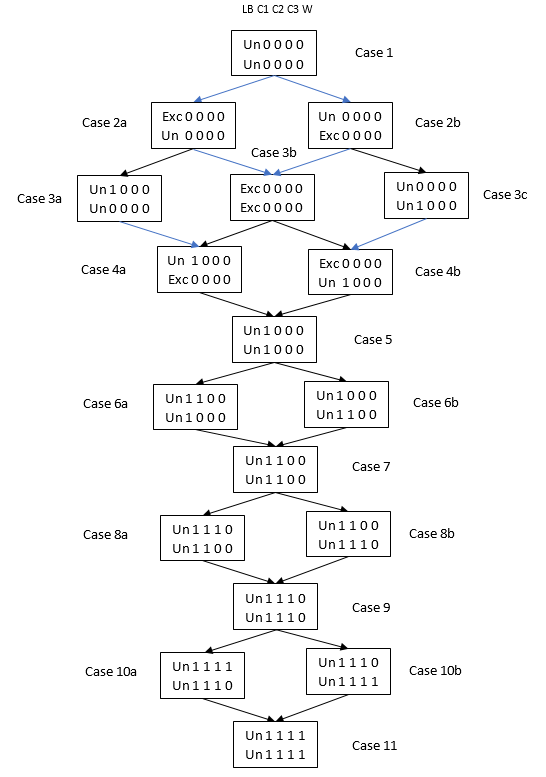
\includegraphics{flowl2c3}
  \caption{The wires in each row are in order of logic block, C1, C2, C3, W.  Each row represents half of the duplicated circuit, ie. top row are A half wires and bottom row are B half wires.  'Un' denotes that the logic block is unexcited and 'Exc' denotes the logic block is excited.  Blue arrows indicate a case change caused by transitions elsewhere in the circuit.  Black arrows indicate a wire transition.}
  \label{fig:l21}
\end{figure}
%fixed 
\begin{lemma}[2.1]
For any state in a trace of the fault tolerant circuit, the wire blocks are in one of the cases in figure \ref{fig:l21}.
\end{lemma}
\begin{proof}
We show by induction that for the fault tolerant circuit, each wire block is in one of the cases in the above figure.  The figure halves the number of cases, as case 11 is the inversion of case 1 (with the 0's and 1's inverted) and from case 11 the state transitions go through the same cases in figure \ref{fig:l21} from 1-11 but inverted.  Thus we only need to analyze possible transitions from each case up to case 10.  Also, Lemma 1 applies to both A half and B half.\\

We look at the base case for every wire $w$ in the original circuit.  Because the duplicated circuit starts at the same valid initial state: $w=c1^A=c2^A=c3^A=w^A=c1^B=c2^B=c3^B=w^B$.  A wire $w$ can be either excited or unexcited in the original circuit. If the wire $w$ is unexcited, applying Lemma 1,  A and B halves of $w$ in the duplicated circuit are in case 1 (or case 11, we will here on ignore the inverted 1's and 0's states, but each case technically represents two states).  If $w$ is excited then Lemma 1 states that the logic blocks must be excited, which is case 2.  Thus this property is true for the base case. \\

In the induction step, assume that the induction hypothesis is true for state $s_k$ and we show that it is true for $s_{k+1}$.  \\

For all possible transitions from $s_k$, we verify that each $s_{k+1}$ has wire blocks that is in one of the cases in figure \ref{fig:l21}.  It is clear that the arrows represent transitions and logic block changes that can occur, thus we are verifying that there does not exist additional cases a transition can lead to, namely that the logic blocks does not behave inappropriately since the wires in the C-element chains behave as the arrows indicate.  Because the arrows do not always indicate wire transitions (some are transitions between excited or unexcited state of the logic blocks which are in response to transitions of other wires), we only need to verify that for the transitions that do occur (black arrows), it does not cause the other logic blocks to behave inappropriately.
\begin{itemize}
\item
Case 1:  Nothing within the wire block can transition.  It is waiting for its input wires to change.  Once a logic block is excited it changes to case 2a or 2b. %this transition needs not occur, 
\item
Case 2a/2b:  In case 2a, $c1^A$ is excited and can transition to case 3a.  Similarly case 2b can transition to case 3c.  From both cases it is possible that the unexcited logic block becomes excited and go to case 3b at the next state.  However the excited logic block cannot become unexcited (without the corresponding $c1$ transition) due to semi-modularity and Lemma 1.
\item
Case 3a/3b/3c:  In case 3a (3c), it is possible for the logic block in B-half (A-half) to become excited, and change to 4a (4b).  The logic block in A-half (B-half) cannot be excited again while $c1^A=1$ ($c1^B=1$) because that violates Lemma 1.  From 3b, when $c1^A$ or $c1^B$ transitions, the next state is 4a or 4b.  The excited logic blocks cannot become unexcited due to semi-modularity and Lemma 1.
\item
Case 4a/4b:
A logic block is excited in both cases and can transition to case 5.  The excited logic block cannot become unexcited due to semi-modularity and Lemma 1.  The already transitioned logic block (unexcited) cannot be excited again due to same reasoning as above (Lemma 1).
\item
%Case 3a/3b:   If a transition occurs in these cases for wire block $w$, the only excited wires are $c1^{B}$ or $c1^{A}$ respectively.  By the same argument as case 2, the excitation state of the 4C-element for all wires in $s_{n+1}$ must remain the same (other than the one that transitions).  Thus in $s_{n+1}$ wire block $w$ is in case 4 while all other wire blocks remains in the same case from $s_n$ and thus all wire blocks are in a case in the figure. \\
Cases 5/6a/6b/7/8a/8b:  In these cases for wire block $w$, the only wires able to transition are the excited C-element wires.  Thus case 5 transitions to case 6a or 6b, cases 6a or 6b transition to case 7, case 7 transitions to case 8a or 8b, and cases 8a or 8b transition to case 9.  The already transitioned logic block (unexcited) cannot be excited again due to same reasoning as above (Lemma 1).
\item
Cases 9/10a/10b:  In cases 1-8a/8b all transitions happen on intermediate wires so the state of the other wire blocks must remain the same.  In cases 9/10a/10b an output/input wire is changed so we must also consider the effects on the other wire blocks.  In case 9, when $w^a$ or $w^b$ is excited and transitions to 10a or 10b, an output wire is changed.  If any logic blocks are in case 9, its logic block cannot change excitations because it would violate Lemma 1.  Thus far, we have shown why the logic blocks in cases 1-9 cannot change excitations other than when drawn in the figure.  The last step is to show that the logic blocks in case 10a or 10b also cannot change excitations.  \\  
We assume that the output wires cannot directly feed back into its logic block so that 10a or 10b cannot cause its own logic block to be excited.  For other logic blocks in case 10a or 10b, a transition in $w^A$ or $w^B$ cannot change the excitation in the other logic blocks.  This is shown by contradiction.  
Assume that there exists another logic block in case 10a and that the $w^A$ transition causes an excitation of wire $v$ in state $s_{k+1}$ (10a and 10b are symmetric so we only have to show for one of them).  In state $s_k$ an output wire mismatch is possible only if it is in cases 10a or 10b.  Thus for all wires $u$ where $u^A\neq u^B$, $c2^A=c2^B$ (which includes $v$).  $w^A$ transitioning does that change the values of those wires so the property is true in state $s_{k+1}$ as well.  It is also true of the newly mismatched wire $w$.  In other words all mismatched wires in $s_{k+1}$ have an output wire that is excited. Then from $s_{k+1}$ there exists a sequence of transitions of the mismatched wires so that they become equal in a later state (other than wire $v$).  In that later state, the excited logic block of $v$ must still be excited due to semi-modularity.  Since the input wires on both halves are equal, the logic block in the other half must be excited while its output wire is excited too.  This violates Lemma 1 and produces a contradiction.  Therefore a transition to 10a or 10b cannot excite the logic blocks in case 10a or 10b in other wire blocks.\\
From case 10a or 10b, there may be a transition to case 11 with a corresponding change in the output wires.  Again this cannot excite logic blocks of wires in case 10a or 10b by repeating the argument above in letting the circuit transition until there are no mismatched wires which contradicts Lemma 1.

%still a slight problem here
\end{itemize}
This shows that all wire blocks in all possible $s_{k+1}$ remain in a case in the figure, and the induction step is complete.\\
By induction on the consecutive states of the trace, the above argument shows that all wire blocks of a fault tolerant circuit are in a case in figure \ref{fig:l21} for all traces. \\
\end{proof}
%may be that I don't need how all the intermediate wires go... but just need the at most one of input excitation and outputs can be mismatched.  But this needs to include if outputs are mismatched then the C-element is the same.... which I think I need to show the signals propagating through??
It is now easy to show that deadlock does not occur since each wire block must be in one of the configurations of figure \ref{fig:l21}.
\begin{lemma}[2.2]
For all traces $\sigma$ in the fault tolerant circuit, deadlock does not occur.
\end{lemma}
\begin{proof}
To show that deadlock does not occur, we show that we can always find an excited wire at any state $s_k$ in a trace of the fault tolerant circuit.  The state $s_k$ can be split into two cases, one is that all output wire pairs in the A half and B half are equal, the second is that there exists at least one wire $v$ such that $v^A\neq v^B$.  In the first case, if every output wire pair are equal, then $h^A(s_n)=h^B(s_n)$ and there exists an excited wire $u$ in the original circuit.  By Lemma 1 both halves of the duplicated circuit for $u$ is excited.  By Lemma 2.1, the circuit must be in case 2-6 for $u$.  In each of these cases at least one wire is excited.  \\
In the second case, for some wire $v$ such that $v^A\neq v^B$, then using Lemma 2.1 wire block $v$ is in case 7a or 7b which has an excited wire, either $v^A$ or $v^B$.  Since there are next transitions for both cases, deadlock does not occur.
\end{proof}

Combining the results of the previous Lemmas shows that the fault tolerant circuit is equivalent to the original circuit under normal operation.  This is defined formally in a theorem as follows:
\begin{theorem}[1]
For all traces $\sigma$ in the fault tolerant circuit, $h^{A}(\sigma_n)$ or $h^{B}(\sigma_n)$ is a prefix of a trace in the original circuit for all $n \in \mathbb{N}$.  (h might make the trace shorter, so the prefix will not be of length n) %what was the point of the deadlock thing?
\end{theorem}
\begin{proof}
Apply Lemma 1 then $h^{A}(\sigma_n)$ or $h^{B}(\sigma_n)$ is a prefix of a trace.  From Lemma 2.2, no deadlock occurs so it is true for all $n\in \mathbb{N}$.
\end{proof}
%with these 3 properties show the original claim
\section{Single transient fault analysis}
%fix this
Next we consider what happens to the fault tolerant circuit under a single transient fault which is defined as follows:
\begin{definition}A transient fault on a wire $w$ causes a transition $w= \lnot w^{prev}$.  After this event it is assumed that the wire can freely transition based on its inputs. %do I need to talk about when transient is not ~x?  ie hold same value?  That's the same as a longer delay
\end{definition}
Next we will show that if a single transient fault occurs on any wire, the fault free half circuit will be equivalent to the original circuit.  Applying Lemma 1, we know that the fault free half will transition according to the original state graph but it may deadlock, so we must prove that it does not deadlock.  To do this we prove some properties that are true when a single transient fault occurs on a wire.  We partition the wires into two sets based on their properties when a single transient fault is added.  Lemma 3 shows that if a single fault occurs on the $c2$ or $c3$ wires for some wire $w$, the output wires still follow the original state graph.  Lemma 4 shows that if a fault occurs to any of the other wires, then the $c2$ or $c3$ wires follow a similar order to the non-fault case and thus the output wire pairs can never be different at deadlock.  Then we combine these Lemmas to show that there is no deadlock.
\begin{lemma}[3]
For all traces $\sigma$ in the duplicated circuit, with a single transient fault occurring on a $c2$ or $c3$ wire of some wire $w$ at any point in the trace, then $h^{A}(\sigma_n)$ and $h^{B}(\sigma_n)$ is a prefix of a trace in the original circuit for all $n \in \mathbb{N}$.
\end{lemma}
\begin{proof}
Without loss of generality we can show this is true if a transient fault occurs in the $A$ half.  We use NuSMV to verify that if a transient fault occurs on one of the $c2$ or $c3$ wires of wire $w$, the input-output characteristic of the local C-element chain do not change.  Under normal operation, by Lemma 2.1 the pair of inputs ($c1^A$, $c1^B$) and outputs ($w^A$, $w^B$) cycle through the wire values shown in figure \ref{fig:l3helper}.  Thus the property verified in NuSMV is that when a single transient fault occurs on wires $c2$ or $c3$, the cycle mentioned previously is always true.    
\begin{figure}
  \centering
    \includegraphics{L3helperfull}
  \caption{The projection of the states in figure \ref{fig:l21} from Lemma 2.1 onto the wires $c1^A$, $c1^B$ and $w^A$, $w^B$.  This forms the input and output characteristic of a wire block under normal operation.}
  \label{fig:l3helper}
\end{figure}

%We first deal with the $0\to 1 \to 0$ fault on $c2^A$.  
We go through an example of a transient on $c3^A$ to demonstrate why this is true.  By Lemma 2.1 the normal circuit will be at some state in figure \ref{fig:l21}, so we analyze the transient occurring at each state in figure \ref{fig:l21}.
\begin{itemize}
	\item
If the current state is 1, 2a, 2b, 3a, 3b, 3c, 4a, 4b, 5, 6a, 6b it does not cause any changes in excitations in the local circuit.  In particular since $w^A$ and $w^B$ do not change, then by semi-modularity the excited/unexcitedness of logic blocks are maintained.  So the transient induced state graph is a copy of the portion containing states 1, 2a, 2b, 3a, 3b, 3c, 4a, 4b only with $c3^A$ value flipped. Eventually they all transition to state 8a and proceed from there as usual.
	\item
If the current state is 7 progresses the state to 8a, the correct transition.	
	\item
      If the current state is 8a then when $c3^A$ experiences a transient, the state
 becomes identical to state 7.  It will then proceed from state 7 as usual.   
	\item
If the circuit experiences a fault in state 9, it will revert back to state 8b.  
	\item
If the circuit experiences a fault in state 10a or 10b, $w_B$ or $w_A$ will go from excited to non excited respectively.  $c3^A$ will be excited but there are no other excitations in the local circuit.  Thus $w^A$ and $w^B$ do not change and by semi-modularity the logic gates to these wires cannot be excited or transition on any subsequent states while $w^A$ and $w^B$ do not change (same argument as in Lemma 2.1 can be used since the other wire blocks do not have transients and thus in one of the states in cases 2.1).  Then the local circuit will stay in this transient induced state until $c3^A$ finally changes and the circuit returns to its state before the transient.
\end{itemize}
%c3
A similar reasoning would then apply if a transient fault occurs in $c1^A$, and also for the $B$ half.  
\end{proof}

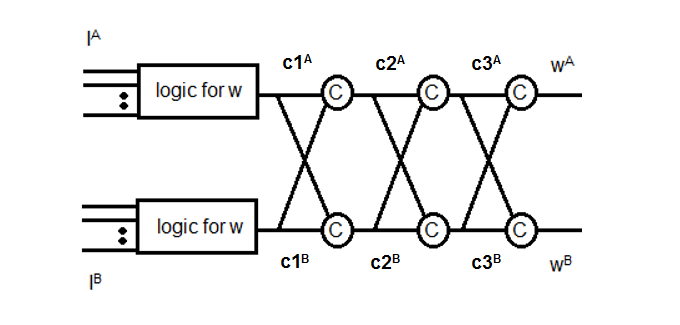
\includegraphics[width=.8\textwidth]{gatew}

\begin{figure}
  \centering
    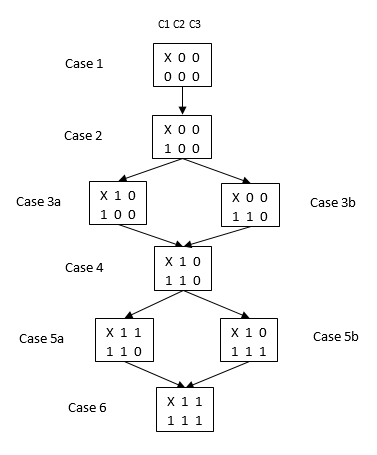
\includegraphics{flowl4c3v2}
  \caption{The wires in each row are in order of $c1$, $c2$ and $c3$.  Each row represents half of the duplicated circuit, ie. top row are A half wires and bottom row are B half wires.  Note that case 5 transitions according to case 1 except with the 0's and 1's inverted.  The states transitions after that are inverted versions of state 2-4 until it transitions back to state 1 (uninverted).}
  \label{fig:l4}
\end{figure}
Next we show that if a fault occurs to any of the other wires, then the $c2$ or $c3$ wires of each wire block of the circuit transitions in a completely predictable pattern analogous to Lemma 2.1.  The main difference is that because a fault may be present we cannot fully predict the value of one of $c1^A$ or $c1^B$.  The following property is true despite not knowing one of the $c1$ wire values and leads to the conclusion that the output wire pairs can never be different at deadlock.  

\begin{lemma}[4]
For all traces $\sigma$ in the fault tolerant circuit, where a fault occurs on a wire other than $c2$ or $c3$, the following property is true: the $c2$ and $c3$ wires of each wire $w\in W$ are always in a state of Figure \ref{fig:l4}.
\end{lemma}
\begin{proof}
Without loss of generality we prove this is true when a fault occurs in the A half.  Then we can assume Lemma 1 is true for the B half.  We show by induction that when the fault is not in $c2$ and $c3$, at any state $s_n$ from the trace $\sigma$, $c1$, $c2$ and $c3$ for all wires $w$ follow the state transitions in figure \ref{fig:l4}.  Again we only analyze for cases 1-5 as 6 onwards behave identically to cases 1-5 except with the 0's and 1's inverted.\\

The base case is for the valid initial state with no faults, projecting the states of figure \ref{fig:l21} from Lemma 2 to just the $c1$, $c2$ and $c3$ wires shows this is true. \\

In the induction step we assume $s_k$ is a state where each wire $w$ is in a case of figure \ref{fig:l4}, then at $s_{k+1}$ we look at the possible next states.  We don't assume anything about the non $c2$ and $c3$ wires for the A-half so that $c1^A$ may change values due to a fault.  However we do expect $c1^A$ to be either a 1 or 0 and that even with hazards on $c1^A$, $c2$ wires transition to either 0 or 1.  We indicate the possibly faulty $c1^A$ by the symbol X.
\begin{itemize}
	\item
Case 1:  $c2$, $c3$ are not excited.  $c1^B$ can be excited depending on the inputs to the logic block.  Therefore, if there is a transition from this state it must be to case 2.
\item
Case 2/3a/3b:  $c2$ can be excited depending on $c1^A$.  $c1^B$ cannot transition to 0 due to Semi-Modularity of wire $w$ and Lemma 1.  Therefore, if there is a transition it must be from case 2 to case 3a or 3b, and case 3a or 3b to case 4.
%I might need to show the excited ness of the good logic gate
\item
Cases 4/5a/5b:  $c1^B$ cannot transition to 0 due to the same reasoning above.  $c2$ is not excited. The only possible transitions are on the $c3$ wires and since there are no faults on them they must transition from case 4 to case 5a or 5b, and from case 5a or 5b to 6.
\end{itemize}
By induction, the property we set out to prove is true, the $c2$ and $c3$ wires will be in a case of figure \ref{fig:l4}. 
The same logic applies to when a fault occurs in the B half and the A half is fault free.  
\end{proof}
The importance of this Lemma is that at most one of $c2$ or $c3$ pairs can be mismatched.  The next theorem shows that this implies all output pairs at deadlock must be equal so there is a possible next condition which contradicts the definition of deadlock.  Thus the fault tolerant circuit does not deadlock under a single transient fault.

%Then the following corollary holds:
%\begin{corollary}[4.2]
%All output pairs at deadlock must be equal
%\end{corollary}

\begin{theorem}[2]
When a single transient fault occurs, if $\sigma$ is a trace in the fault tolerant circuit, then one of $h^{A}(\sigma_n)$ or $h^{B}(\sigma_n)$ (the non faulty half) for all $n \in \mathbb{N}$ is a prefix of a trace in the original circuit.  And the circuit does not deadlock.  
\end{theorem}
\begin{proof}
Without loss of generality we can assume the fault occurs in the A half of the circuit.  First by Lemma 3 we know that if the fault occurs on $c2$ or $c3$ wire the circuit does not deadlock.  Thus we only look at when the fault occurs on all other wires. 
Next, we prove that a deadlocked circuit in this scheme must have at least one pair of output wires which have different values.  That is $w^A\neq w^B$ for some wire $w$.
This is shown by contradiction.  Assume that the circuit is deadlocked at state $s$ and $v^A = v^B$ for all wires $v$ from the original circuit.  If a transient occurs, one can wait until that wire is free to transition.  There
 must be a wire $w$ that is excited in the state $h^B(s)$ in the original circuit and we look at that wire block in the duplicated circuit.  We examine each case in Lemma 4.
\begin{itemize}
	\item
	Case 1: Since $w$ is excited then by Lemma 1 $c1^B$ or $w^B$ must be excited and can transition.
\item
Case 2:  $c1^A$ may be 0 or 1.  If $c1^A=0$, since the inputs to A half and B half are equal then $c1^A$ must be excited and can transition to 1.  If $c1^A=1$ then it can transition to case 3a or 3b.
\item
Case 3a/3b:  $c1^A$ may be 0 or 1.  If $c1^A=0$, since the inputs to A half and B half are equal then $c1^A$ must be excited and can transition to 1.  If $c1^A=1$ then it can transition to case 4.
\item
Case 4/5a/5b:  $c3$ is excited and can transition.
\end{itemize}
Thus a transition can always occur and the circuit is not deadlocked which leads to a contradiction.  To remain deadlocked, it must be true that there exists a wire where $w^A\neq w^B$, which implies its $c1^A\neq c1^B$ and $c2^A\neq c2^B$ and $c3^A\neq c3^B$.  But we have shown in Lemma 4 that $c2^A\neq c2^B$ and $c3^A\neq c3^B$ cannot occur at the same time under a single transient fault. Thus deadlock is not possible.  And applying Lemma 1, $h^B(\sigma_n)$ is a prefix of a trace in the original circuit. 
\end{proof}

\bibliography{biblio}
\bibliographystyle{unsrt}
%\bibliographystyle{plain}

%\begin{thebibliography}{9} %9 if number of items between 0-9, 99 if 10-99 etc
%\bibitem{digitaltesting1} 
%N. K. Jha and S. Gupta,
%\textit{Testing of Digital Systems}. 
%Cambridge: Cambridge University Press, 2003.

%\end{thebibliography}
\end{document}